\title{Designing a Minimum Distance to Class Mean Classifier\\}

\author{\IEEEauthorblockN{Md. Mukitul Islam (140204076)}
\IEEEauthorblockA{\textit{Dept. of Computer Science \& Engineering} \\
\textit{Ahsanullah University of Science \& Technology}\\}
}

\maketitle


\section{Objective}
Objective of this experiment is to design a “Minimum Distance to Class Mean Classifier” to classify unclassified sample vectors with the help of some given classified sample vectors.

\section{Introduction}
“Minimum Distance to Class Mean Classifier” is used to classify unclassified sample vectors where the vectors clustered in more than one classes. For example, in a dataset of n sample vectors of dimension d, if some of the sample vectors are already clustered into classes and if some are not classified than we can use this classifier to classify the unknown vectors.\\
In our dataset 12 samples are classified in two different classes and 4 samples are not classified. We have used this minimum distance to class mean classifier that we have implemented to classify those 4 unclassified samples.

\section{Experimental design and Implementation }
For designing a minimum distance to class mean classifier we have used some classified sample vectors and for testing purpose we have used some unclassified sample. 
\subsection{Description of the Experimental Parameters}
We have used the following two-class set of prototypes-\\
$w1$ = {(2,2), (3,1), (3,3), (-1,-3), (4,2), (-2,-2)}\\
$w2$ = {(0,0), (-2,2), (-1,-1), (-4,2), (-4,3), (2,6)}\\
These are the classified sample points we have used in this experiment to design this classifier.\\
For testing purpose we have used the following points-\\
$X_{1}$ = (-1,-1)\\
$X_{2}$ = ( 3, 2)\\
$X_{3}$ = (-2, 1)\\
$X_{4}$ = ( 8, 2)\\
We have classified this points either in class $w1$ or $w2$ based on the decision of this classifier.

\subsection{Class Mean \& Distance Calculations}
For determining class mean we have use MATLAB defined function $mean()$~\cite{b1}. In this $mean()$ function we pass the values of class $w1$ and $w2$ and it returns their class mean value respectively.
\begin{figure}[ht]
\begin{minipage}[c]{\linewidth}
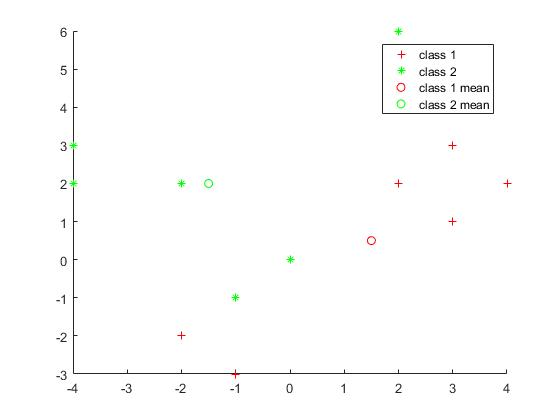
\includegraphics[height=.9\linewidth,width=\linewidth]{classmean.jpg}
\caption{Class 1 \& Class 2 points with their Class Mean}
\end{minipage}
\end{figure}
In the figure red circle signifies the mean of class 1 and green circle signifies the mean of class 2. For plotting all these points we have used MATLAB defined function $plot()$.~\cite{b1}
\\
Distance calculation for a testing point from each class mean-\\
Let us consider, there is $i$ classes and $u_{1},u_{2},.....u_{i}$ be the class mean of each class respectively and there is $i$ unknown samples $x_{1},x_{2},.....x_{i}$, we have to calculate the distance from each class of these samples. For distance calculation we have used Euclidean distance calculation method.
Let, $D_{i}$ be the distance from $ith$ class-\\
\[D_{i}=\sqrt{\left ( x_{1}-u_{1} \right )^2+\left ( x_{2}-u_{2} \right )^2+....+\left ( x_{i}-u_{i} \right )^2}\]\\
\[or,D_{i}^2={\left ( x_{1}-u_{1} \right )^2+\left ( x_{2}-u_{2} \right )^2+....+\left ( x_{i}-u_{i} \right )^2}\]\\
\[or,D_{i}^2={\left ( x - u \right )^t\left ( x - u \right )}\]\\
\[or,D_{i}^2={x^t x-x^t u-u^t x+u^t u}\]\\
\[or,D_{i}^2={x^t x-2u^t x+u^t u}\]\\
\[or,D_{i}^2={-2u^t x+u^t u}\]\\
\[or,-\frac{1}{2}D_{i}^2={u^t x-\frac{1}{2}u^t u} \label{eq:distance} \tag{1}\]

Here,\eqref{eq:distance} gives us the distance of any unclassified sample $x$ from the class mean $u$ of $ith$ class.

\subsection{Decision Rule \& Algorithm Implementation}
In this problem there are 2 classes - $w1$ and $w2$. We have to generate a discriminant function to make decision rule.\\
Discriminant function for $ith$ class-\\
\[
    g_{i}\left ( x\right )=-\frac{1}{2}D_{i}^2={u^t x-\frac{1}{2}u^t u} \label{eq:ge} \tag{2}\\
\]
So, for class $w1$ and $w2$ we have got discriminant function $g_{1}$ and $g_{2}$ respectively. Using this discriminant function we can make the decision rule.\\
Here, the decision rule is-\\

if $g_{1}\left ( x\right ) > g_{2}\left ( x\right )$ then $x \varepsilon w1$

if $g_{1}\left ( x\right ) < g_{2}\left ( x\right )$ then $x \varepsilon w2$

Using these two decision rule this algorithm classifies any unknown sample $x$ to class either $w1$ or $w2$.\\
\begin{figure}[ht]
\begin{minipage}[c]{\linewidth}
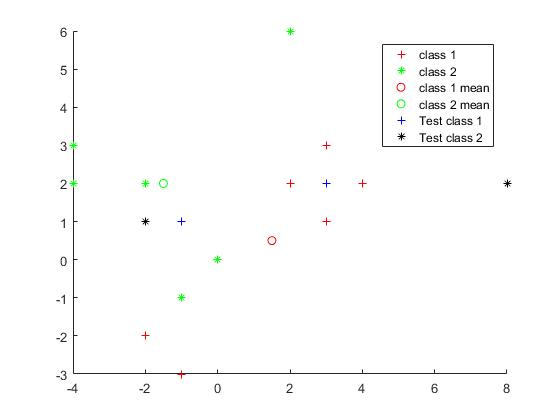
\includegraphics[height=.9\linewidth,width=\linewidth]{testpoint.jpg}
\caption{Class 1 \& Class 2 points with Classified Testing Points}
\end{minipage}
\end{figure}
In this figure, sample of 12 points from class 1 and class 2 are represented by '+' and '*' marker respectively. Plot of four testing points are also in this figure. These four points are also represented with the same marker but with different color. Four testing points are classified here according to the decision rule we have implemented.
\subsection{Decision Boundary}
The two discriminant function can be used to generate the formula for the decision boundary of the two classes $w1$ and $w2$.
For decision boundary,\\
\[
    g_{1} - g_{2} = 0
\]
\[or,
    \left ( u_{1} - u_{2} \right )x - \frac{1}{2}\left\{ u_{1}^t u_{1} - u_{2}^t u_{2}\right\} = 0 \label{db}\tag{3}
\]

Here, \eqref{db} gives us the decision boundary of the two class $w1$ and $w2$.

\section{Result Analysis}
In our dataset there are 12 samples for training purpose these are classified samples and there are 4 samples for testing and these unclassified.
\begin{figure}[ht]
\begin{minipage}[c]{\linewidth}
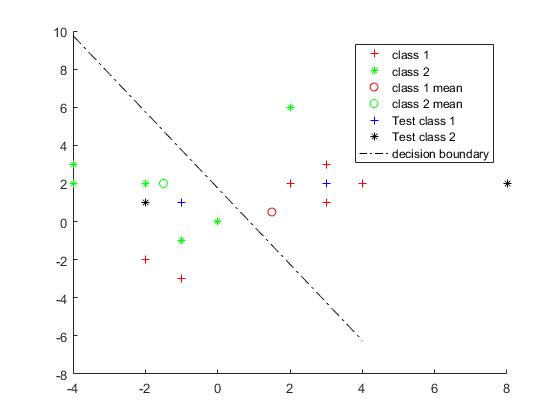
\includegraphics[height=.9\linewidth,width=\linewidth]{final.jpg}
\caption{Class 1 \& Class 2 points with Decision Boundary}
\end{minipage}
\end{figure}
From these figure we can see that among the four testing points, 2 of them classified properly and for two occasions the classifier is failed and misclassified two points. So, accuracy is 50\% for the dataset and testing points we have used here.

\section{Conclusion}
This algorithm is a very simple algorithm and easy to implement and apply. As it conducts simple calculations, its’ calculation is apparently faster. The weakness of the algorithm is its misclassification rate is also relatively higher because the boundary between the two classes is linear.

\begin{thebibliography}{00}
\bibitem{b1}
MATLAB Documentations,
\textit{https://www.mathworks.com/}
\end{thebibliography}
